% SC2000 — Chapter 8: Hypothesis Testing & Linear Regression
\chapter{Hypothesis Testing \& Linear Regression}
\label{ch:hypothesis}

\begin{quote}
\emph{``You cannot prove a hypothesis; you can only fail to reject it.''} Does the new cache policy really reduce miss rate? Is latency correlated with load? Hypothesis testing turns these questions into decisions with controlled error rates; regression quantifies the relationship.
\end{quote}

\noindent\fbox{\parbox{\dimexpr\linewidth-2\fboxsep-2\fboxrule}{%
\textbf{From zero: decisions under uncertainty.} We formalise null vs.\ alternative, $p$-values, Type~I/II errors, then build $z$/$t$/$\chi^2$ tests and simple linear regression from least squares---all with computing examples.}}
\vspace{0.4em}

\section*{Learning Outcomes}
After this chapter you will be able to:
\begin{enumerate}[label=(L\arabic*)]
    \item formulate $H_0$ vs.\ $H_1$, choose a test statistic, and compute $p$-values;
    \item control Type~I/II errors, power, and significance level $\alpha$;
    \item apply $z$-, $t$-, and $\chi^2$ tests for means, proportions, and goodness-of-fit;
    \item derive and interpret simple linear regression (least squares, $R^2$);
    \item run one-way ANOVA to compare three or more means via the $F$-test;
    \item diagnose $p$-hacking, multiple testing, and practical vs.\ statistical significance.
\end{enumerate}

% ============================================================
\section{The Logic of Hypothesis Testing}
\label{sec:logic-testing}
We have data $X_1,\dots,X_n$ and two competing claims:

\begin{definition}[Hypotheses] \emph{Null} $H_0$ (status quo, e.g., $\mu=\mu_0$) vs.\ \emph{alternative} $H_1$ (what we seek evidence for: $\mu\ne\mu_0$, $\mu>\mu_0$, or $\mu<\mu_0$). A \emph{test} is a rule: reject $H_0$ if test statistic $T(X)$ falls in a critical region.
\end{definition}

\begin{definition}[$p$-value] $p=P_{H_0}(T\text{ at least as extreme as observed})$. Small $p$ = data surprising under $H_0$. Reject $H_0$ if $p\le\alpha$ (significance level, e.g., $0.05$).
\end{definition}

\begin{definition}[Errors] Type~I: reject $H_0$ when true (rate $\alpha$). Type~II: fail to reject when $H_1$ true (rate $\beta$). \emph{Power} $=1-\beta=P_{H_1}(\text{reject})$. Increasing $n$ or effect size raises power.
\end{definition}

\emph{Court analogy:} $H_0=$ innocent, $H_1=$ guilty. Type~I $=$ convict innocent; Type~II $=$ acquit guilty. ``Not guilty'' $\ne$ ``innocent''---failing to reject $H_0$ does not prove it.

\begin{figure}[h]
\centering
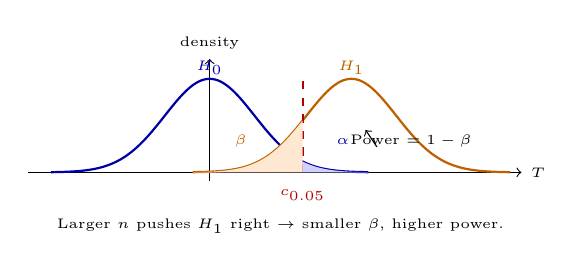
\begin{tikzpicture}[scale=0.72,every node/.style={font=\scriptsize}]
% Two normals: H0 at 0, H1 at 2.5, with alpha region and beta region
\draw[->,thin] (-3.2,0)--(5.5,0) node[right,font=\tiny] {$T$};
\draw[->,thin] (0,-0.15)--(0,2.0) node[above,font=\tiny] {density};
% H0 curve at 0
\draw[thick,blue!65!black,smooth,domain=-2.8:2.8,samples=60] plot (\x,{1.65*exp(-\x*\x/1.25)});
\node[font=\tiny,blue!65!black] at (0,1.85) {$H_0$};
% H1 curve at 2.5
\draw[thick,orange!75!black,smooth,domain=-0.3:5.3,samples=60] plot (\x,{1.65*exp(-(\x-2.5)*(\x-2.5)/1.25)});
\node[font=\tiny,orange!75!black] at (2.5,1.85) {$H_1$};
% critical value at 1.64 (alpha=0.05 one-sided)
\draw[dashed,thick,red!70!black] (1.64,0)--(1.64,1.75);
\node[font=\tiny,red!70!black] at (1.64,-0.40) {$c_{0.05}$};
% alpha shading (H0 tail beyond c)
\fill[blue!18] (1.64,0) -- plot[domain=1.64:2.8,samples=30] (\x,{1.65*exp(-\x*\x/1.25)}) -- (2.8,0) -- cycle;
\node[font=\tiny,blue!65!black] at (2.35,0.55) {$\alpha$};
% beta shading (H1 mass before c)
\fill[orange!18] (-0.3,0) -- plot[domain=-0.3:1.64,samples=30] (\x,{1.65*exp(-(\x-2.5)*(\x-2.5)/1.25)}) -- (1.64,0) -- cycle;
\node[font=\tiny,orange!75!black] at (0.55,0.55) {$\beta$};
% power = 1-beta
\node[font=\tiny,align=center] at (3.55,0.55) {Power $=1-\beta$};
\draw[->,thin] (2.95,0.45)--(2.75,0.75);
\node[font=\tiny,align=center] at (1.25,-0.95) {Larger $n$ pushes $H_1$ right $\to$ smaller $\beta$, higher power.};
\end{tikzpicture}
\caption{Null ($H_0$, blue) vs.\ alternative ($H_1$, orange) densities for test statistic $T$. Critical value $c$ leaves $\alpha$ in $H_0$'s tail; $\beta$ is $H_1$'s mass before $c$; power $=1-\beta$.}
\label{fig:errors-power}
\end{figure}

% ============================================================
\section{Tests for Means and Proportions}
\label{sec:tests-means}

\paragraph{$z$-test (large $n$ or known $\sigma$).} $Z=(\bar X-\mu_0)/(\sigma/\sqrt{n})\approx\mathcal{N}(0,1)$ under $H_0$. Two-sided $p=2(1-\Phi(|z_{\text{obs}}|))$.

\paragraph{$t$-test (small $n$, Normal data, unknown $\sigma$).} $T=(\bar X-\mu_0)/(S/\sqrt{n})\sim t_{n-1}$ under $H_0$. Use $t$ critical values.

\paragraph{Proportion test.} $\hat p=S/n$, $Z=(\hat p-p_0)/\sqrt{p_0(1-p_0)/n}\approx\mathcal{N}(0,1)$.

\paragraph{Two-sample $t$-test.} Compare means $\mu_1,\mu_2$ via $\bar X_1-\bar X_2$ with pooled or Welch $t$.

\begin{example}[Cache policy] Old miss rate $12\%$ ($p_0=0.12$). New policy: $98$ misses in $1000$ accesses ($\hat p=0.098$). $z=(0.098-0.12)/\sqrt{0.12\cdot0.88/1000}=-2.14$, $p=0.032<0.05$: reject $H_0$, new policy significantly better (at $5\%$).
\end{example}

\subsection{$\chi^2$ Goodness-of-Fit}
Test if data follow a hypothesised distribution: $\chi^2=\sum_{i=1}^k(O_i-E_i)^2/E_i\approx\chi^2_{k-1}$ under $H_0$. E.g., is a die fair? Is packet size distribution Poisson?

% ============================================================
\section{Simple Linear Regression}
\label{sec:regression}
We model $Y_i=\beta_0+\beta_1 x_i+\varepsilon_i$, $\varepsilon_i\sim\mathcal{N}(0,\sigma^2)$ (or just mean $0$, var $\sigma^2$ for least squares).

\begin{definition}[Least squares] Choose $\hat\beta_0,\hat\beta_1$ minimising $\sum_{i=1}^n(Y_i-\beta_0-\beta_1x_i)^2$.
\end{definition}

Solution:
\[
\hat\beta_1=\frac{\sum(x_i-\bar x)(Y_i-\bar Y)}{\sum(x_i-\bar x)^2}=\frac{\widehat{\mathrm{Cov}}(x,Y)}{\widehat{\mathrm{Var}}(x)},\qquad
\hat\beta_0=\bar Y-\hat\beta_1\bar x.
\]
Fitted values $\hat Y_i=\hat\beta_0+\hat\beta_1x_i$, residuals $e_i=Y_i-\hat Y_i$.

\begin{definition}[$R^2$] $R^2=1-\frac{\sum e_i^2}{\sum(Y_i-\bar Y)^2}\in[0,1]$, fraction of variance explained. $R^2=r_{xY}^2$ (squared correlation) in simple regression.
\end{definition}

\begin{figure}[h]
\centering
\begin{tikzpicture}[scale=0.72,every node/.style={font=\scriptsize}]
\draw[->,thick] (-0.3,0)--(5.2,0) node[right,font=\tiny] {$x$ (e.g., load)};
\draw[->,thick] (0,-0.3)--(0,4.2) node[above,font=\tiny] {$Y$ (e.g., latency)};
% data points
\foreach \x/\y in {0.6/0.85,1.1/1.35,1.6/1.55,2.0/2.25,2.45/2.55,2.9/3.05,3.4/3.35,3.9/3.85,4.4/4.05} {
  \fill[blue!65!black] (\x,\y) circle (2.2pt);
}
% regression line
\draw[thick,red!70!black] (0.2,0.55)--(4.8,4.35);
\node[font=\tiny,red!70!black] at (4.85,4.15) {$\hat Y=\hat\beta_0+\hat\beta_1x$};
% residuals as dashed verticals for two points
\draw[dashed,thin,orange!75!black] (2.0,2.25)--(2.0,1.95);
\draw[dashed,thin,orange!75!black] (2.9,3.05)--(2.9,2.75);
\node[font=\tiny,orange!75!black] at (2.0,2.55) {$e_i$};
% R2 annotation
\node[font=\tiny,align=center,fill=green!10,rounded corners=2pt,inner sep=3pt] at (1.15,3.85) {$R^2=1-\dfrac{\text{RSS}}{\text{TSS}}$\\fraction explained};
\end{tikzpicture}
\caption{Simple linear regression: best-fit line minimises sum of squared residuals (dashed). $R^2$ measures how much $Y$ variation the line explains.}
\label{fig:regression}
\end{figure}

\begin{figure}[h]
\centering
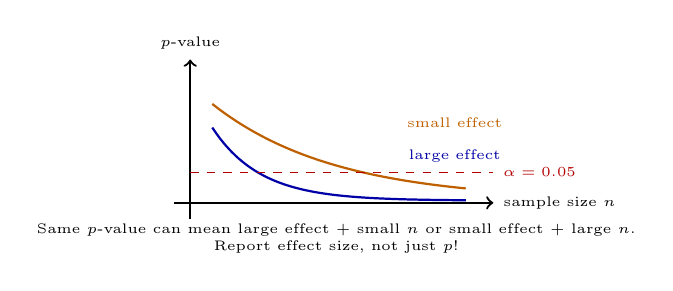
\begin{tikzpicture}[scale=0.70,every node/.style={font=\scriptsize}]
% p-value dance: effect size vs sample size
\draw[->,thick] (0,-0.3)--(0,2.6) node[above,font=\tiny] {$p$-value};
\draw[->,thick] (-0.3,0)--(5.5,0) node[right,font=\tiny] {sample size $n$};
% large effect: p drops fast
\draw[thick,blue!65!black,smooth,domain=0.4:5,samples=40] plot (\x,{2.1*exp(-\x*1.15)+0.04});
\node[font=\tiny,blue!65!black] at (4.8,0.85) {large effect};
% small effect: p drops slowly
\draw[thick,orange!75!black,smooth,domain=0.4:5,samples=40] plot (\x,{2.1*exp(-\x*0.45)+0.04});
\node[font=\tiny,orange!75!black] at (4.8,1.45) {small effect};
% alpha line
\draw[dashed,red!70!black] (0,0.55)--(5.5,0.55) node[right,font=\tiny] {$\alpha=0.05$};
\node[font=\tiny,align=center] at (2.65,-0.65) {Same $p$-value can mean large effect + small $n$ or small effect + large $n$.\\Report effect size, not just $p$!};
\end{tikzpicture}
\caption{$p$-values conflate effect size and sample size. A tiny $p$ with huge $n$ may reflect a practically irrelevant effect---always report confidence intervals and effect sizes.}
\label{fig:pvalue-effect}
\end{figure}

Inference: under Normal errors, $\hat\beta_1\sim\mathcal{N}(\beta_1,\sigma^2/\sum(x_i-\bar x)^2)$, giving CI and $t$-test for $H_0:\beta_1=0$ (``is there a linear relationship?'').

% ============================================================
\section{One-Way ANOVA: Comparing Several Means}
\label{sec:anova}
\emph{Intuition:} with $g\ge3$ groups, pairwise $t$-tests multiply false positives. ANOVA asks one question instead: is the spread \emph{between} group means large compared with the noise \emph{within} groups? Total variation splits additively: $\mathrm{SST}=\mathrm{SSB}+\mathrm{SSW}$. The $F$ statistic $F=\frac{\mathrm{SSB}/(g-1)}{\mathrm{SSW}/(n-g)}$ sits near $1$ when all means agree and grows when some group stands out; under $H_0$ (equal means, Normal noise) $F\sim F_{g-1,n-g}$.
\begin{example}[Worked] Three schedulers, $4$ latency runs each: group means $41,44,50$, grand mean $45$. $\mathrm{SSB}=4[(41-45)^2+(44-45)^2+(50-45)^2]=4(16+1+25)=168$; within-group $\mathrm{SSW}=60$. $F=\frac{168/2}{60/9}=\frac{84}{6.67}=12.6>F_{2,9,0.95}=4.26$: reject $H_0$ --- some scheduler differs. Follow up with pairwise tests (Bonferroni) to find which one.
\end{example}

% ============================================================
\section{Caveats: $p$-Hacking and Practical Significance}
\label{sec:caveats}
\emph{Multiple testing:} $20$ tests at $\alpha=0.05$ give $\approx64\%$ chance of a false positive. Correct via Bonferroni ($\alpha/k$) or FDR (Benjamini--Hochberg). \emph{$p$-hacking:} trying many analyses until $p<0.05$ invalidates $p$. Pre-register hypotheses. \emph{Practical vs.\ statistical:} with $n=10^6$, a $0.01\%$ improvement can be ``significant'' yet useless. Always report effect size and CI.

% ============================================================
\section{Computing Tests \& Regression in Code}
\label{sec:code-testing}

\begin{lstlisting}[language=Python]
import math, random

def z_test_proportion(phat, p0, n):
    se = math.sqrt(p0*(1-p0)/n)
    z = (phat - p0)/se
    # two-sided p-value via erf
    Phi = lambda x: 0.5*(1+math.erf(x/math.sqrt(2)))
    pval = 2*(1 - Phi(abs(z)))
    return z, pval

z, pval = z_test_proportion(0.098, 0.12, 1000)
print(f"z={z:.2f} p={pval:.4f} {'reject H0' if pval<0.05 else 'fail to reject'}")

# Simple linear regression (closed form)
def linreg(x, y):
    n = len(x)
    mx, my = sum(x)/n, sum(y)/n
    Sxx = sum((xi-mx)**2 for xi in x)
    Sxy = sum((xi-mx)*(yi-my) for xi, yi in zip(x, y))
    b1 = Sxy / Sxx
    b0 = my - b1*mx
    yhat = [b0 + b1*xi for xi in x]
    RSS = sum((yi-yh)**2 for yi, yh in zip(y, yhat))
    TSS = sum((yi-my)**2 for yi in y)
    R2 = 1 - RSS/TSS
    return b0, b1, R2

x = [1,2,3,4,5,6,7,8]
y = [2.1,3.9,6.2,7.8,10.1,11.9,14.2,16.0]
print("beta0,beta1,R2 =", linreg(x, y))
\end{lstlisting}

% ============================================================
\section{Chapter Notes}
Neyman--Pearson (1933) formalised testing; Fisher advocated $p$-values. The replication crisis (Ioannidis 2005, Open Science Collaboration 2015) exposed $p$-hacking; modern guidance (ASA 2016, 2019) urges abandoning ``$p<0.05$'' as a bright line. Regression is Gauss (1809) and Legendre (1805); see Freedman \emph{Statistical Models} for pitfalls and Simpson's paradox (Ch.~3) as regression confounding.

% ============================================================
\section{Exercises}
\label{sec:ch08-exercises}
\begin{enumerate}[label=E8.\arabic*, leftmargin=*, itemsep=0.8em]
\item \textbf{$z$-test.} $n=64$ packet delays give $\bar x=48.2\,$ms, $\sigma=8\,$ms known. Test $H_0:\mu=50$ vs.\ $H_1:\mu\ne50$ at $\alpha=0.05$. Compute $z$, $p$, decision, and $95\%$ CI. Do CI and test agree?
\item \textbf{Power.} For $H_0:\mu=0$ vs.\ $H_1:\mu=0.5$ with $\sigma=1$, $n=25$, one-sided $\alpha=0.05$, compute power. How large must $n$ be for power $\ge0.80$?
\item \textbf{$\chi^2$ fairness.} A die rolled $60$ times gives counts $[7,12,9,14,6,12]$. Test fairness at $\alpha=0.05$ ($\chi^2_{5,0.95}=11.07$). Compute $\chi^2$ statistic and decide.
\item \textbf{Regression by hand.} Data $(x,y)$: $(1,2),(2,3),(3,5),(4,4),(5,6)$. Compute $\hat\beta_0,\hat\beta_1,R^2$ via formulas. Predict at $x=6$ and give a residual plot interpretation.
\item \textbf{Multiple testing.} $100$ independent true-null tests at $\alpha=0.05$. What is $P(\text{at least one false positive})$? What Bonferroni $\alpha$ controls family-wise error at $0.05$? Why is FDR less conservative?
\end{enumerate}
% End of Chapter 8
